\section{Angebot und Bedarf}
\label{sec:Angebot und Bedarf}
\subsection{a}
Anhand eines Datensatzes von monatlichen Einstrahlungsdaten für den Zeitraum von 2011-2020, welcher der Datenbank PVGIS entnommen worden ist \cite{PVGIS}, konnten Jahressummen für den Standort Berlin ermittelt werden.\\
Der Mittelwert der Jahressummen wurde im Folgenden als jährliche horizontale Globalstrahlungssumme verwendet.
Für diesen Wert wurden die Differenzen zu der kleinsten und größten Jahressumme errechnet.
Die größere Differenz wird als worst-case angenommen und als Toleranz $\Delta E$ festgelegt.
Diese erste Berechnung ergibt eine durchschnittliche jährliche Einstrahlungssumme
auf der Horizontalen von $E = 1132,465 \frac{kWh}{m^2\cdot a} \pm 111,055 \frac{kWh}{m^2\cdot a}$.\\
Anhand der vorgegebnen Süd-Ost-Aurichtung und dem Neigungswinkel von 45° kann aus dem untenstehenden Diagramm der Umrechnungs- bzw. Ausrichtungsfaktor abglesen werden.\\
Dieser beträgt in diesem Fall 1,05, somit ergibt sich auf der geneigten Kollektorebene eine jährliche Einstrahlungssumme von
$E_{gen} = 1189,088 \frac{kWh}{m^2\cdot a} \pm 116,608 \frac{kWh}{m^2\cdot a}$.

\begin{figure}[H]
  \centering
  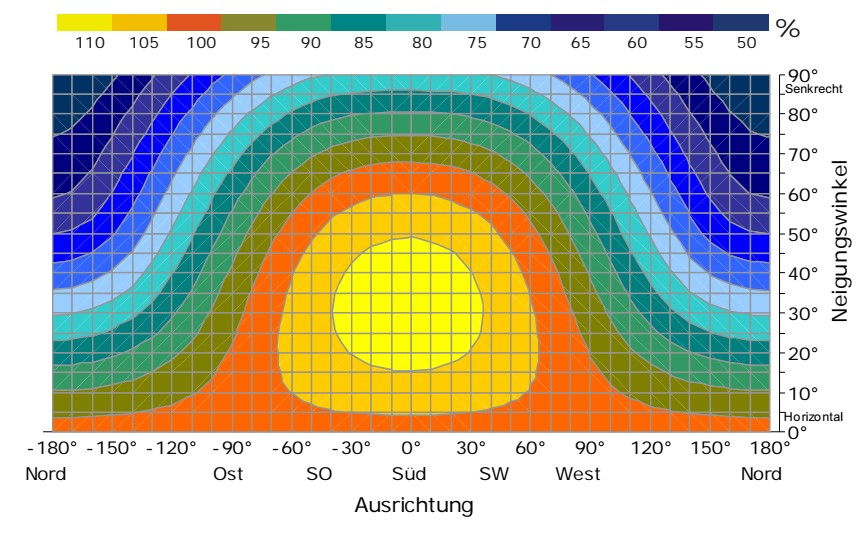
\includegraphics[width=\textwidth]{Abbildungen/Ausrichtung.jpg}
  \caption{Änderung der jährlichen solaren Bestrahlung in Berlin in Abhängigkeit von Ausrichtung
  und Neigung im Vergleich zur Horizontalen \cite[S.92]{QUA19}}
  \label{fig:Ausrichtungsfaktor}
\end{figure}